\subsection{Carga y Materia}

Todo lo que nos rodea, como una pelota, el aire, una planta o nuestro propio cuerpo, está formado por \textbf{átomos}. Los átomos, a su vez, están compuestos por tres tipos de partículas: \textbf{protones, neutrones y electrones}. Los protones y neutrones se encuentran en el núcleo del átomo, mientras que los electrones se mueven alrededor en la corteza. Los protones tienen \hl{carga positiva}, los electrones \hl{carga negativa}, y los neutrones no tienen carga. 

\begin{figure}[ht]
    \centering
    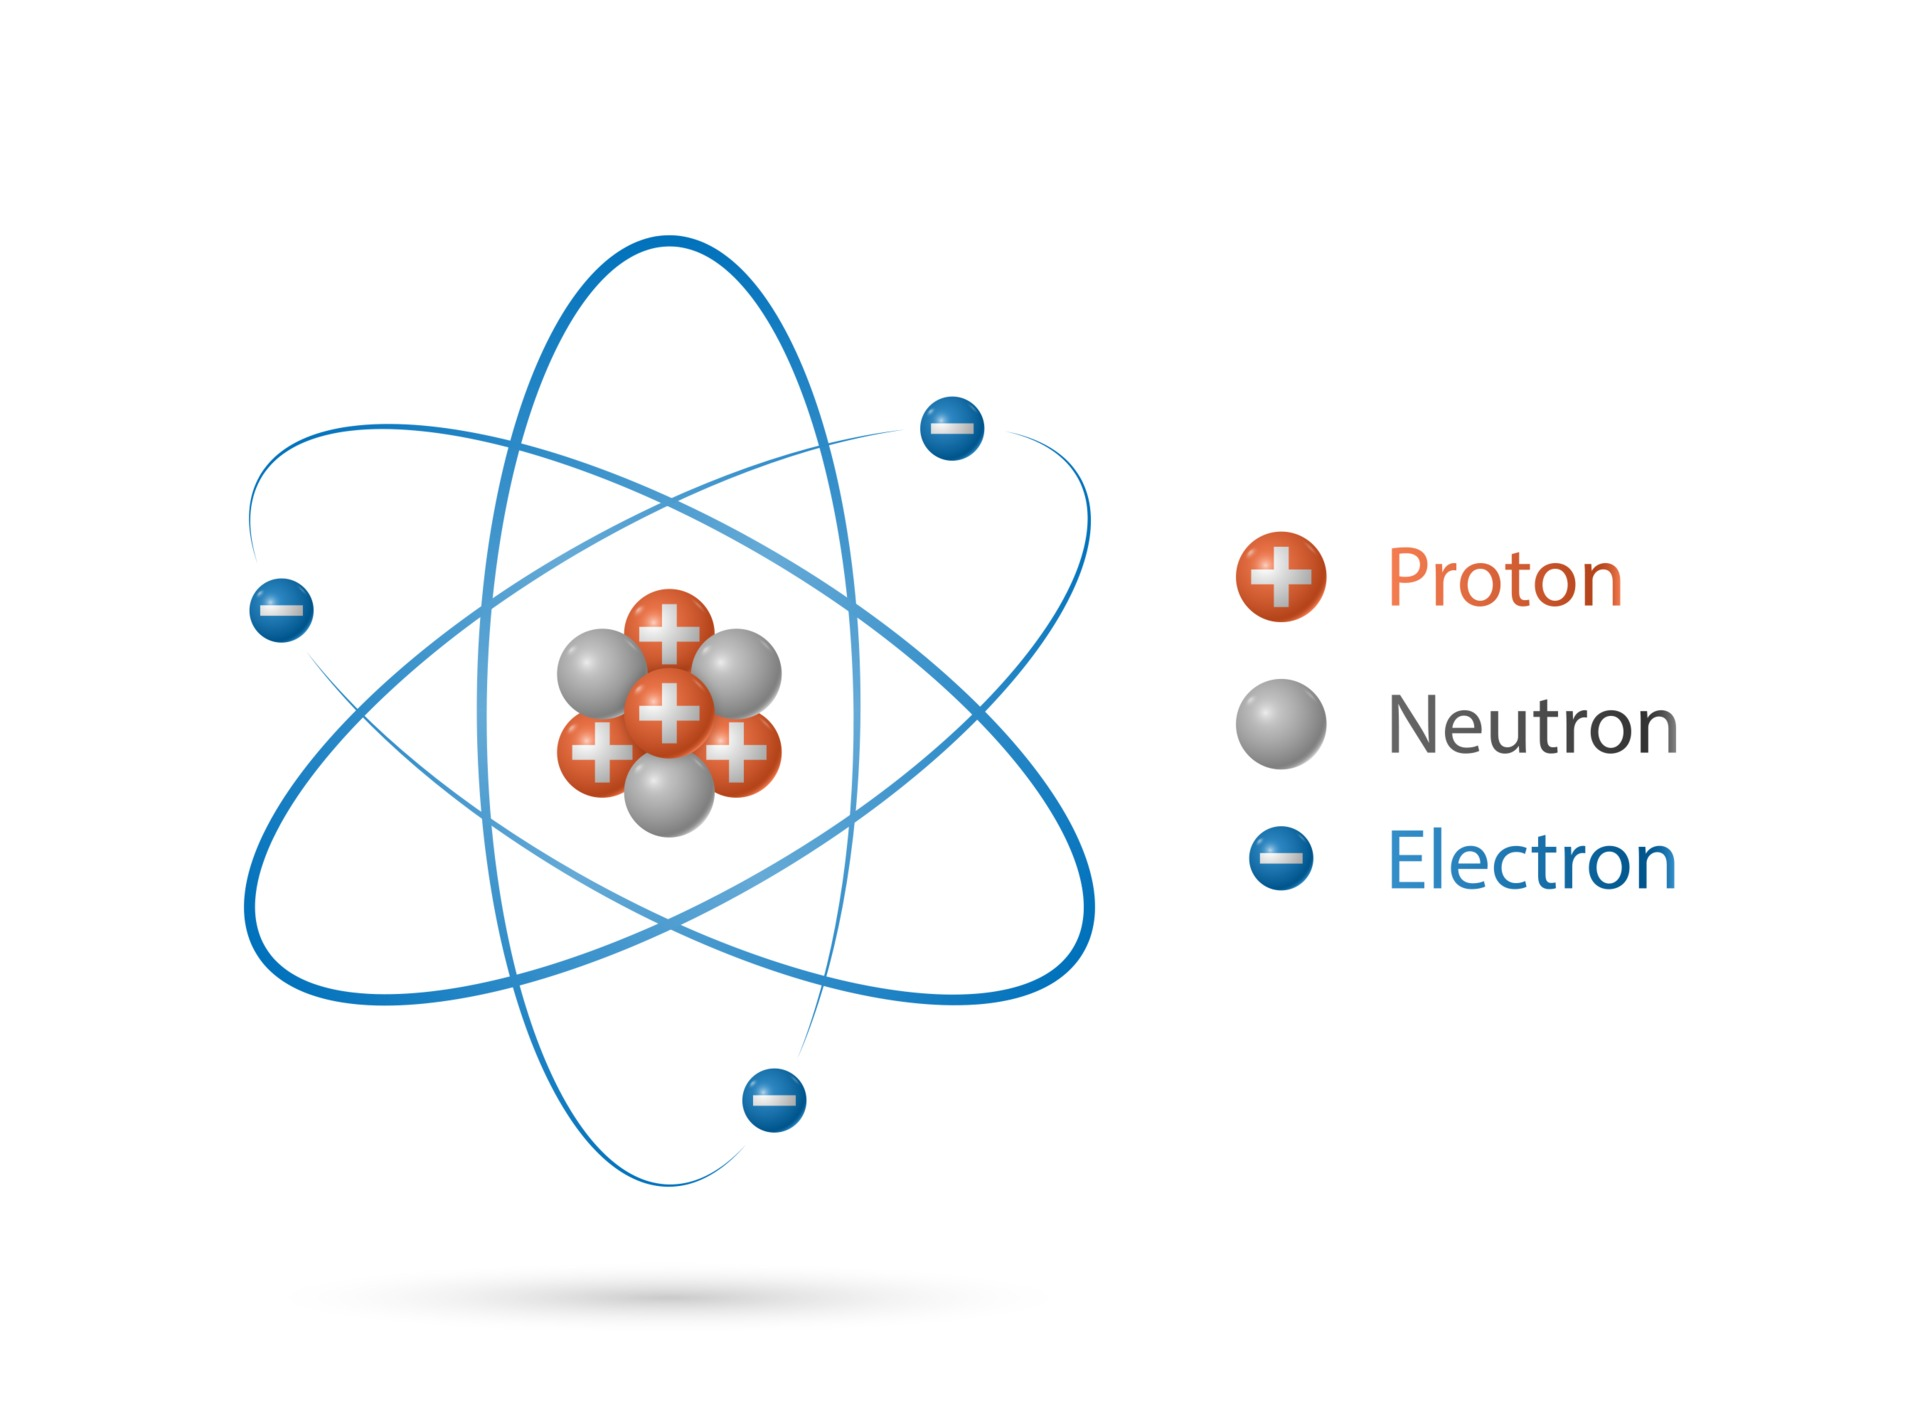
\includegraphics[width=0.4\textwidth]{atom_struct.jpg}
    \caption{Estructura básica de un átomo.}
    \label{fig:atom_struct}
\end{figure}

Esta estructura corresponde a un \textbf{modelo atómico}, que es una representación que nos ayuda a entender cómo está compuesto un átomo y cómo se comporta. A lo largo del tiempo han existido distintos modelos atómicos, pero uno de los más conocidos es el \textbf{modelo de Bohr}. Según este modelo, los electrones giran alrededor del núcleo en \textbf{órbitas circulares}, cada una con un nivel de energía específico. Cuando un electrón cambia de órbita, absorbe o emite energía en forma de luz.

La carga elemental \colorbox{highlight}{\( e \)} es la \textbf{cantidad más pequeña de carga eléctrica libre que se conoce en la naturaleza}. Es la carga que poseen los protones y electrones, pero con signo opuesto:
\begin{itemize}
    \item \textbf{Electrón}: \( -e = -1.602 \times 10^{-19} \) C (coulombs)
    \item \textbf{Protón}: \( +e = 1.602 \times 10^{-19} \) C
\end{itemize}

La carga elemental es fundamental porque todas las cargas eléctricas observadas en la naturaleza son \textbf{múltiplos enteros de \( e \)}. Es decir, cualquier carga presente en un objeto es el resultado de un exceso o déficit de electrones. Este principio se conoce como la \textbf{ley de conservación de la carga eléctrica}, y establece que la carga eléctrica \textbf{no se crea ni se destruye}, solo se transfiere de un cuerpo a otro.  

Los objetos tienen carga debido a la presencia de \textbf{electrones y protones}. Un objeto es eléctricamente neutro cuando tiene igual número de ambos. Si un objeto adquiere carga negativa, significa que ha \textbf{ganado electrones}, y si adquiere carga positiva, significa que ha \textbf{perdido electrones}. Cuando un objeto se carga, no se están creando nuevas cargas, sino que \textbf{se están moviendo electrones} de un cuerpo a otro. Por ejemplo: en la \textbf{electrización por frotamiento}, un material transfiere electrones a otro, dejando uno cargado positivamente y el otro negativamente. En la \textbf{inducción}, un objeto cargado puede redistribuir las cargas en otro sin tocarlo, pero sin cambiar la cantidad total de carga en el sistema.

En otras palabras, la carga eléctrica siempre se conserva porque \textbf{los electrones y protones no se destruyen en procesos normales}, solo cambian de ubicación dentro de un sistema.

\colorbox{highlight}{Denominaremos con la letra \( Q \) o \( q \) a la carga eléctrica de un objeto.} La carga se mide en \textbf{coulombs (C)}. Un coulomb es una cantidad de carga muy grande, por lo que en la práctica se utilizan submúltiplos como el \textbf{milicoulomb (mC)} o el \textbf{microcoulomb (\( \mu \text{C} \))}.